\chapter{Listings test}

Here is a little test how a listing part might be shown ...

%\lstset{style=listingstyle}
%\lstinputlisting[language=c++]{./listings/main.cpp}
\newpage

\section{Base Station}

\lstinputlisting[language=c++,style=listingstyle]{../../LcsNodes-Pico/LcsBaseStation/LcsBaseStation.h}
\newpage

\lstinputlisting[language=c++,style=listingstyle]{../../LcsNodes-Pico/LcsBaseStation/LcsBsCommand.cpp}
\newpage

\lstinputlisting[language=c++,style=listingstyle]{../../LcsNodes-Pico/LcsBaseStation/LcsBsDccTrack.cpp}
\newpage

\lstinputlisting[language=c++,style=listingstyle]{../../LcsNodes-Pico/LcsBaseStation/LcsBsLocoSession.cpp}
\newpage

\lstinputlisting[language=c++,style=listingstyle]{../../LcsNodes-Pico/LcsBaseStation/main.cpp}
\newpage

\section{CDC Lib}

\lstinputlisting[language=c++,style=listingstyle]{../../LcsNodes-Pico/LcsLibraries/LcsCdcLib/LcsCdcLib.h}
\newpage

\lstinputlisting[language=c++,style=listingstyle]{../../LcsNodes-Pico/LcsLibraries/LcsCdcLib/LcsCdcLib.cpp}
\newpage

First attempt ...

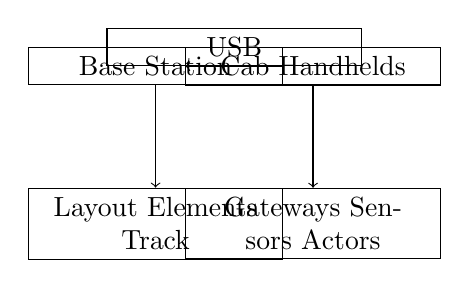
\begin{tikzpicture}[node distance=2cm, every node/.style={draw, text width=3cm, align=center}]
% Nodes
\node (base) {Base Station};
\node[right of=base] (cab) {Cab Handhelds};
\node[below of=cab] (gateways) {Gateways Sensors Actors};
\node[below of=base] (track) {Layout Elements \\ Track};

% Arrows
\draw[->] (base) -- (cab) node[midway, above] {USB};
\draw[->] (cab) -- (gateways);
\draw[->] (base) -- (track);

\end{tikzpicture}
